\subsection{Mapping for a Solenoid in Lab}

The magnetic field $B$ generated in section \ref{sec:FieldGeneration}, yielded to the following figures. In this particular set of measurements the main objective is to capture the spatial gradient behavior of an static magnetic field produced by a solenoid, which has a constant current flow throughout the experiment. Figure \ref{fig:bfield_time_z} shows two plots from the field mapped, Fig. \ref{fig:bfield_time} shows the magnetic field flux B in gauss as a function of time going in and out to the solenoid front face, while Fig. \ref{fig:bfield_z} shows the estimated respective positions of the probe along the z-axis.


\begin{figure}[hbt!]
	\centering
	\subfigure[$B$ field as a function of time.\label{fig:bfield_time}]{
		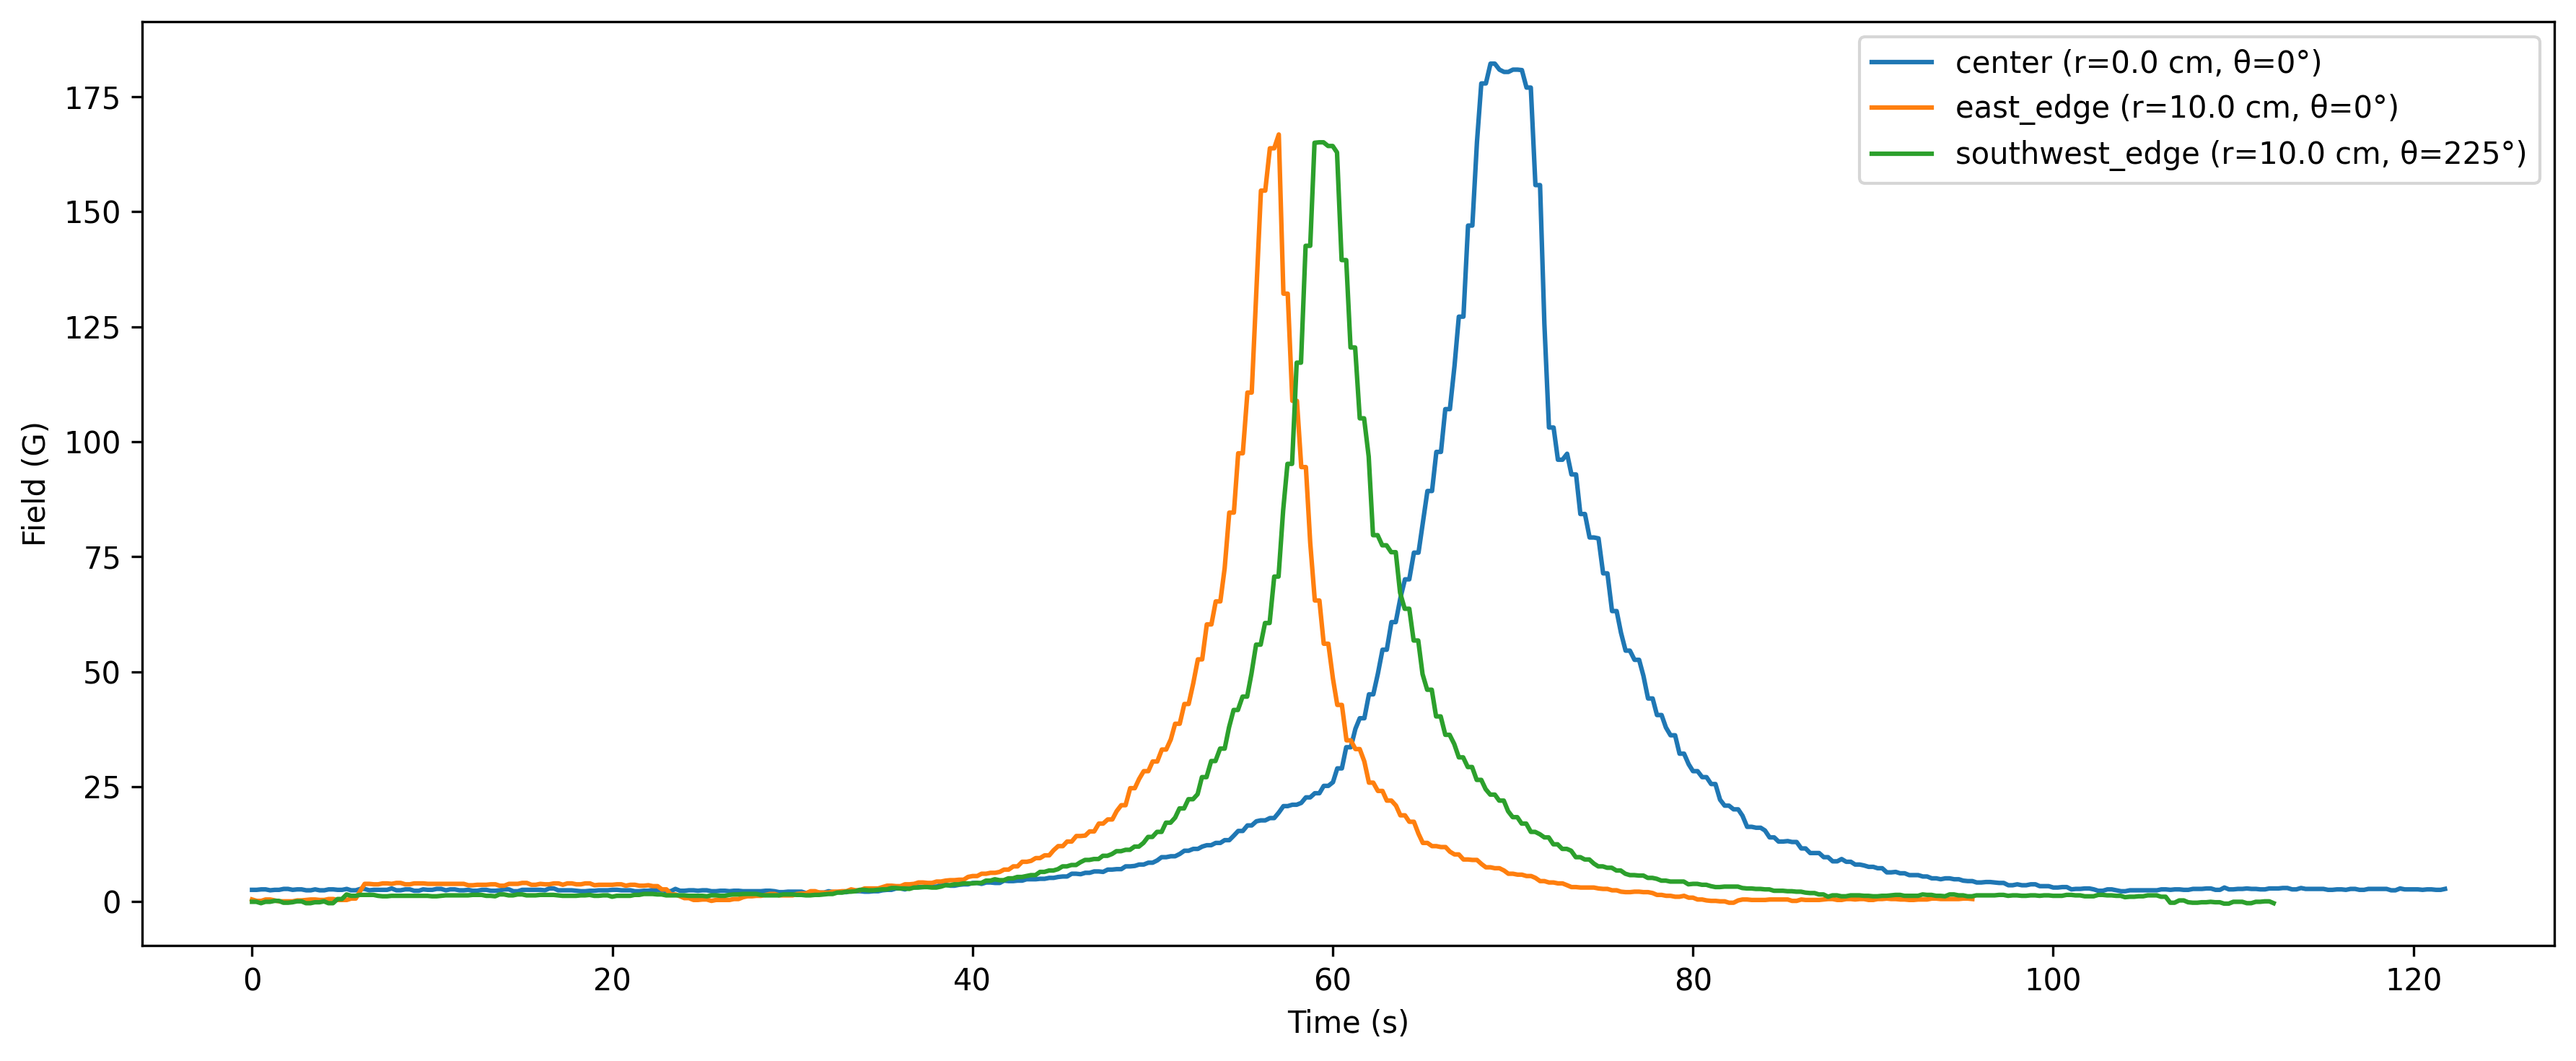
\includegraphics[width=0.9\textwidth]{Assets/BfieldvsTime.png}
	}
	\hfill
	\subfigure[$B$ field as a function of $z$-position.\label{fig:bfield_z}]{
		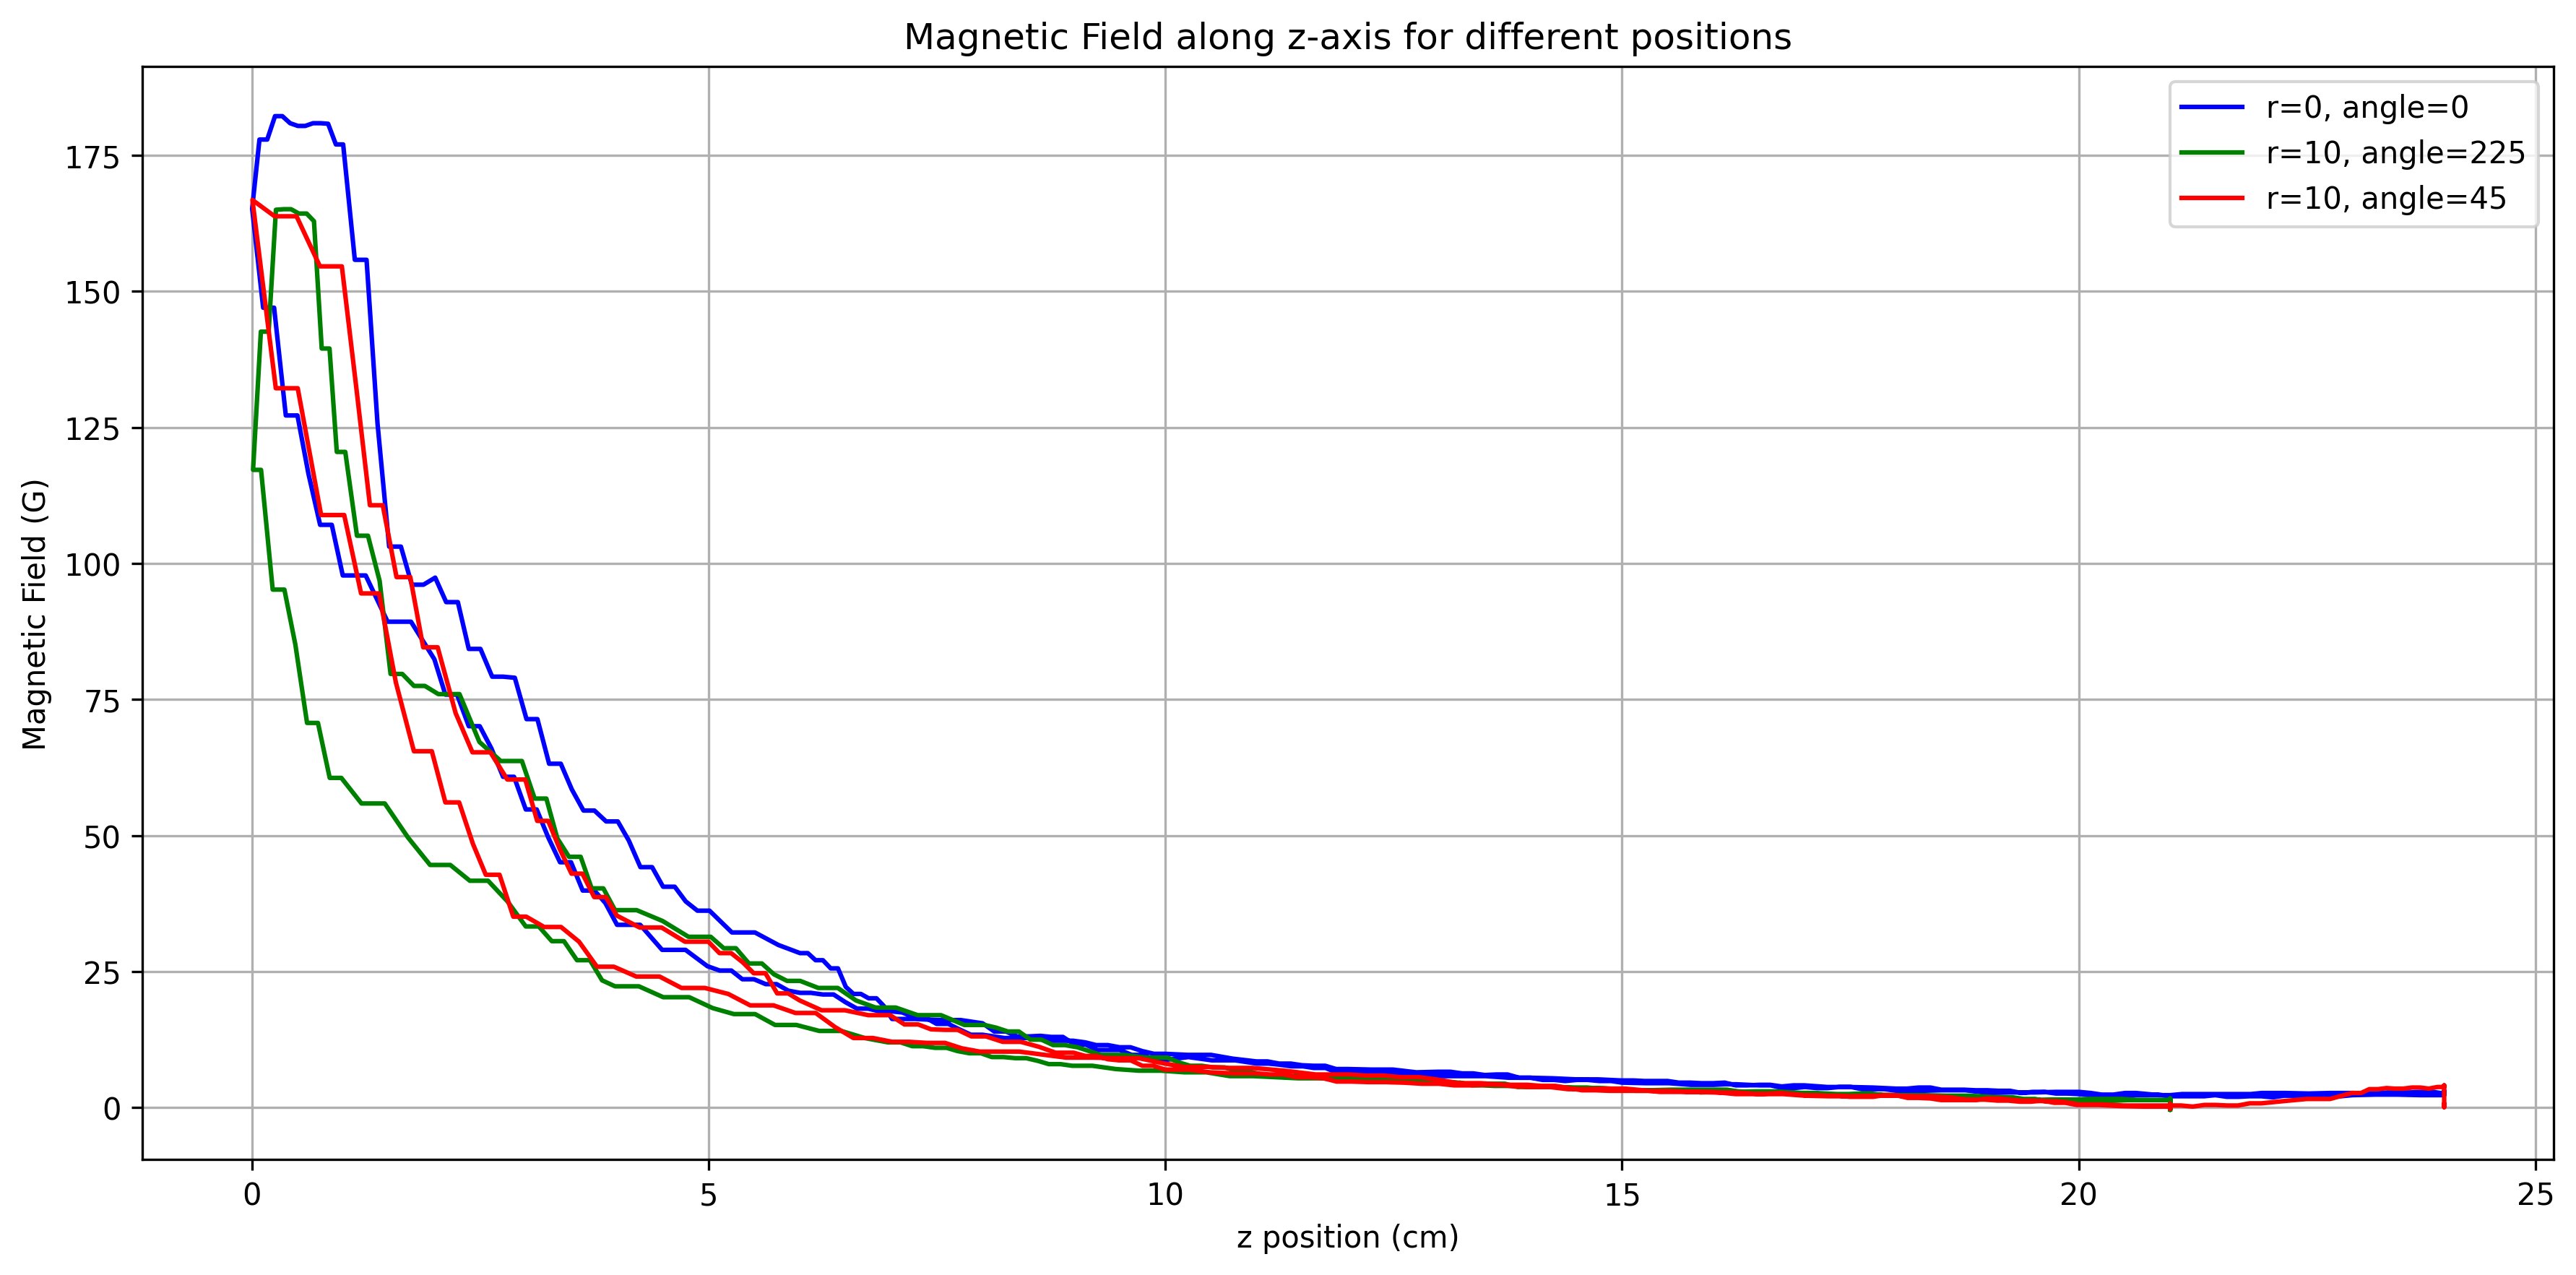
\includegraphics[width=0.8\textwidth]{Assets/BfieldvsZ.png}
	}
	
	\caption[$B$-field behavior along time and displacement]{Magnetic field measurements plotted against time and axial displacement. Used to estimate stability and spatial variation of the mapping setup.}
	\label{fig:bfield_time_z}
\end{figure}

The three colors represent the position of the probe on each trial, this can be seen clearly on Figure \ref{fig:bfield3d} where the map was plotted as a representative line for their respective side. It is important to notice the similarities between runs on the southwest side and the east side of the front as this expected homogeneity allow us to extrapolate the data around the solenoid similar to Fig \ref{fig:3D_field_plot} confirming the theoretical background and speeding our clinical magnetic field acquisition protocol.


\begin{figure}[htb!]
	\centering
	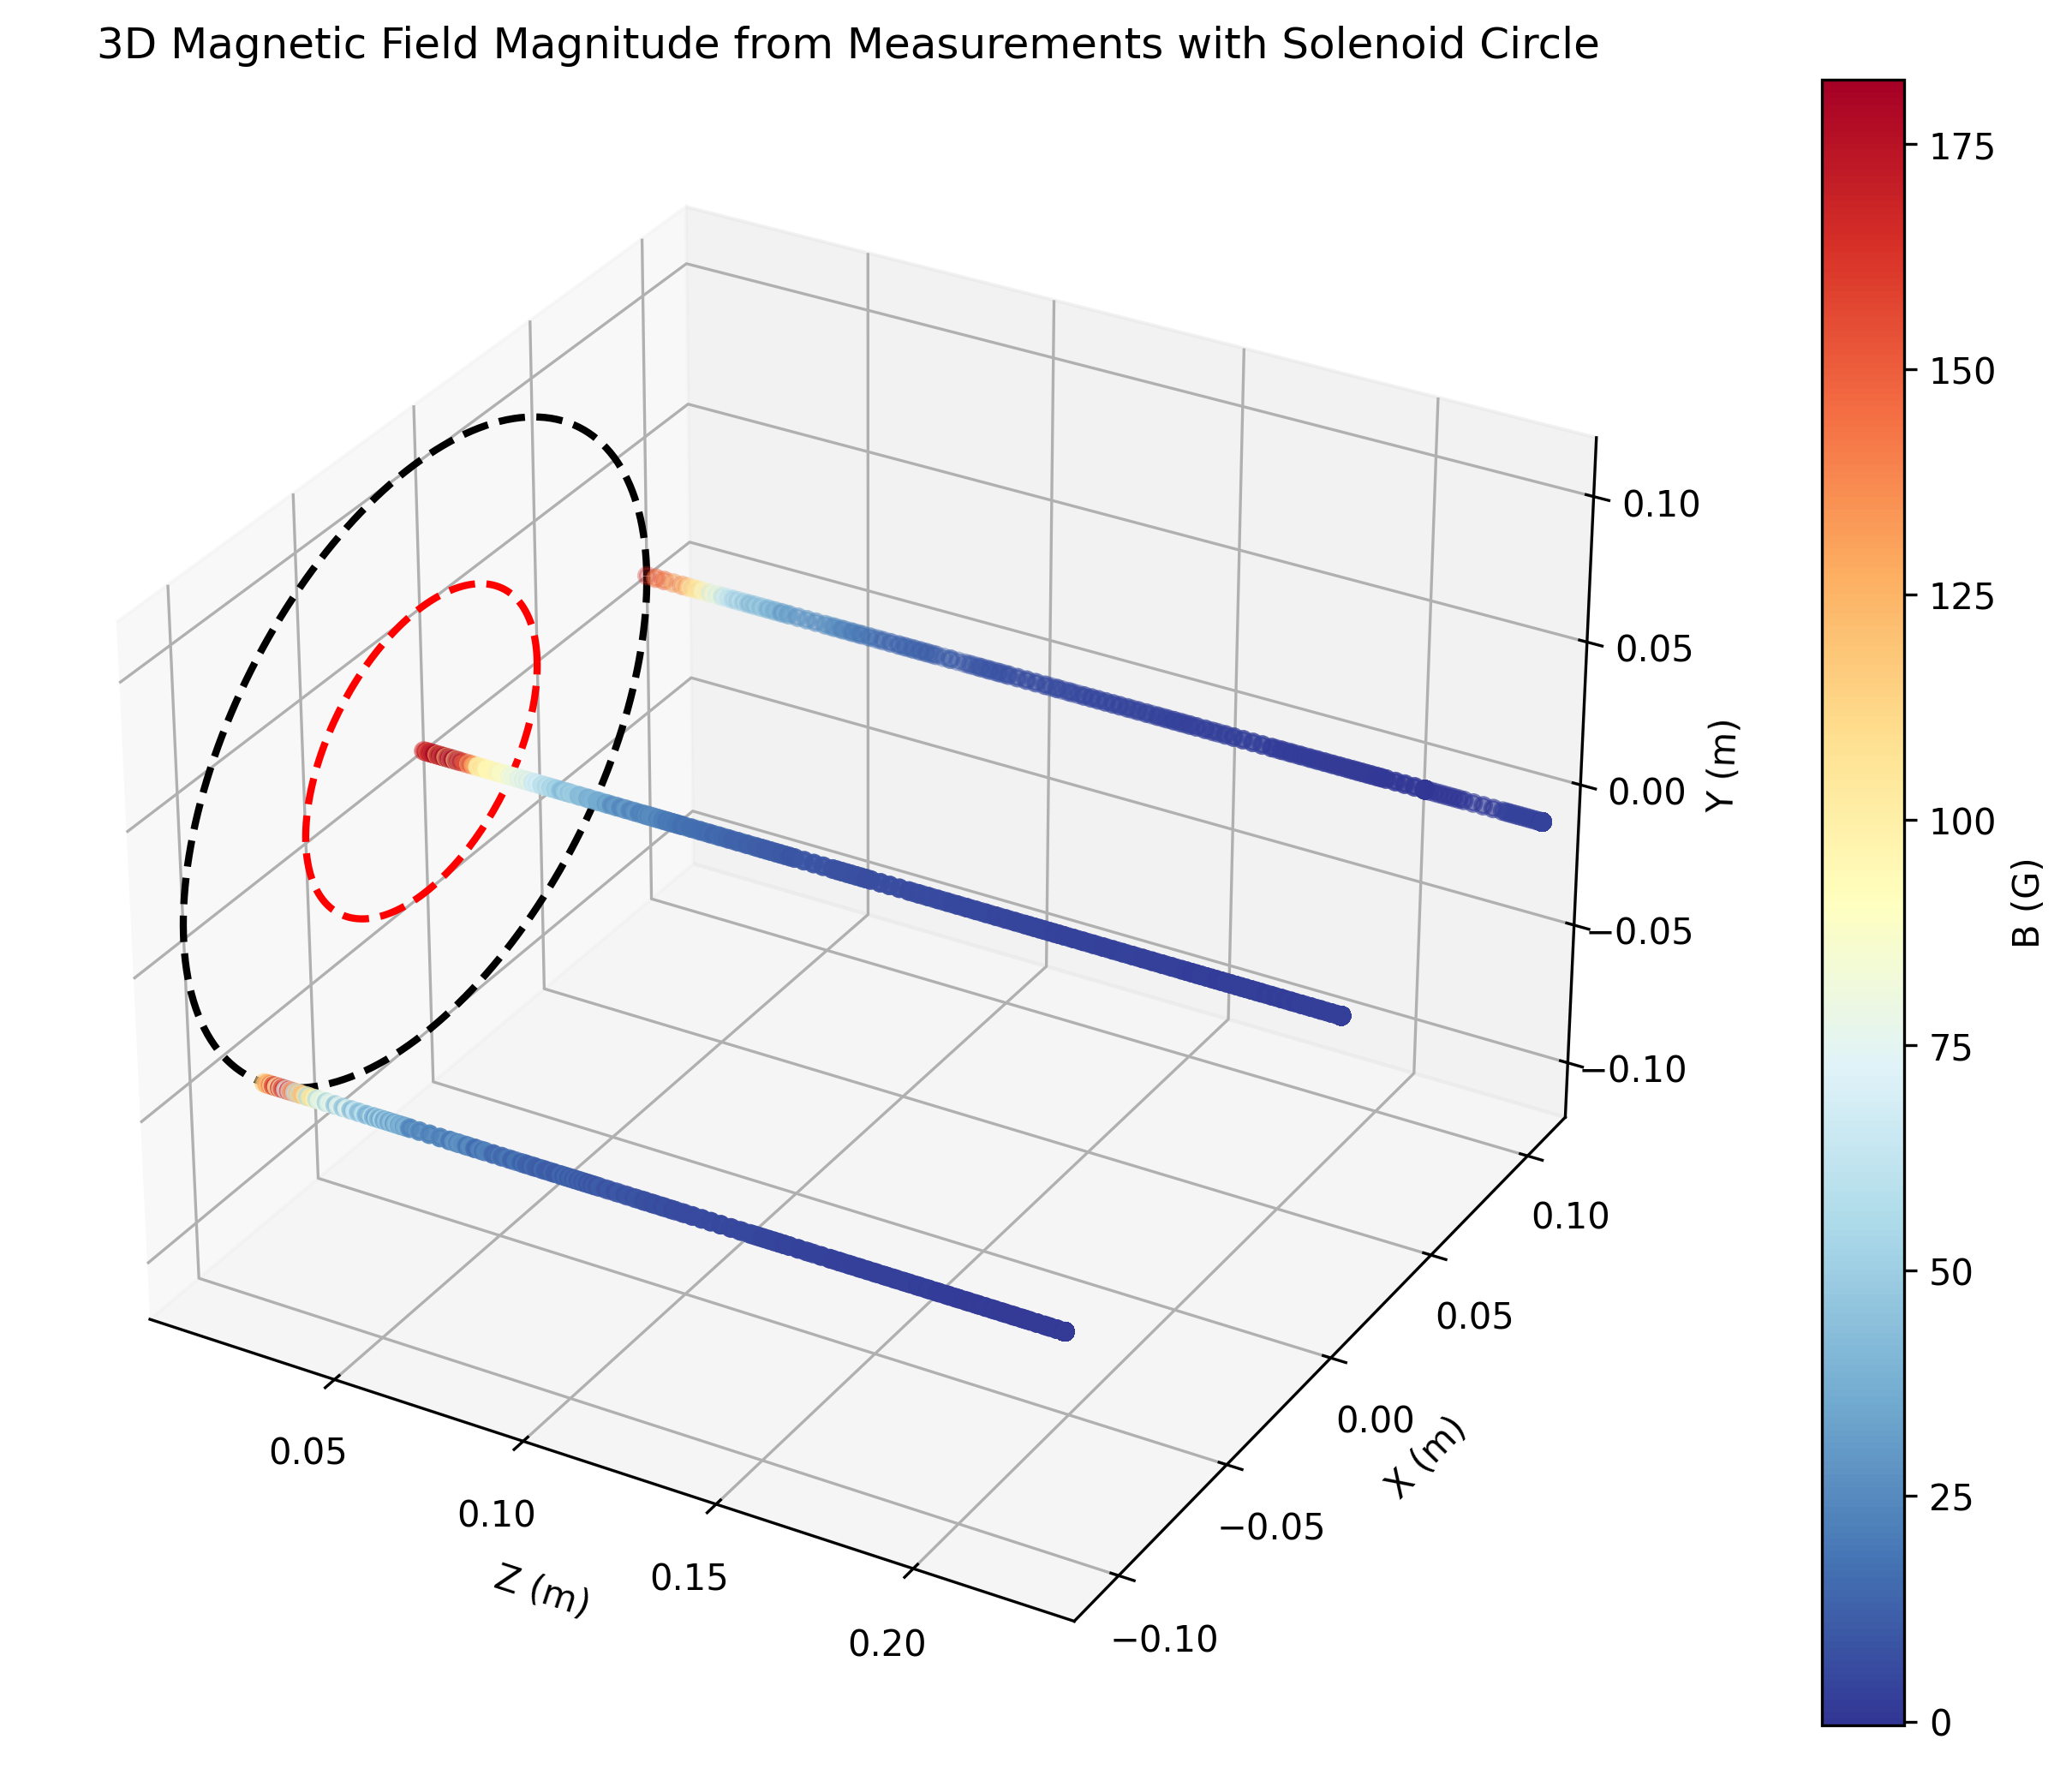
\includegraphics[width=0.75\textwidth]{Assets/Bfield3dreal.png}
	\caption[3D reconstructed field map]{Three-dimensional reconstruction of the measured magnetic field, illustrating spatial variation across the mapping region.}
	\label{fig:bfield3d}
\end{figure}

Figure \ref{fig:gradb_pair} shows both the calculated gradient from equation \ref{eq:finiteDiff}, and the multiplication by field strength $B$ at the particular current of 2.966 A. The later being useful on experiment \ref{sec:Translational} for finding magnetic force, as per equation \ref{eq:translationalForce}, and for its fit (see Eq.\ref{eq:forFit}) making one point out of the set in the translational experiment described in section \ref{sec:experiment1}.

\begin{figure}[hbt!]
	\centering
	\subfigure[$\nabla B$ along the measurement path.\label{fig:gradb}]{
		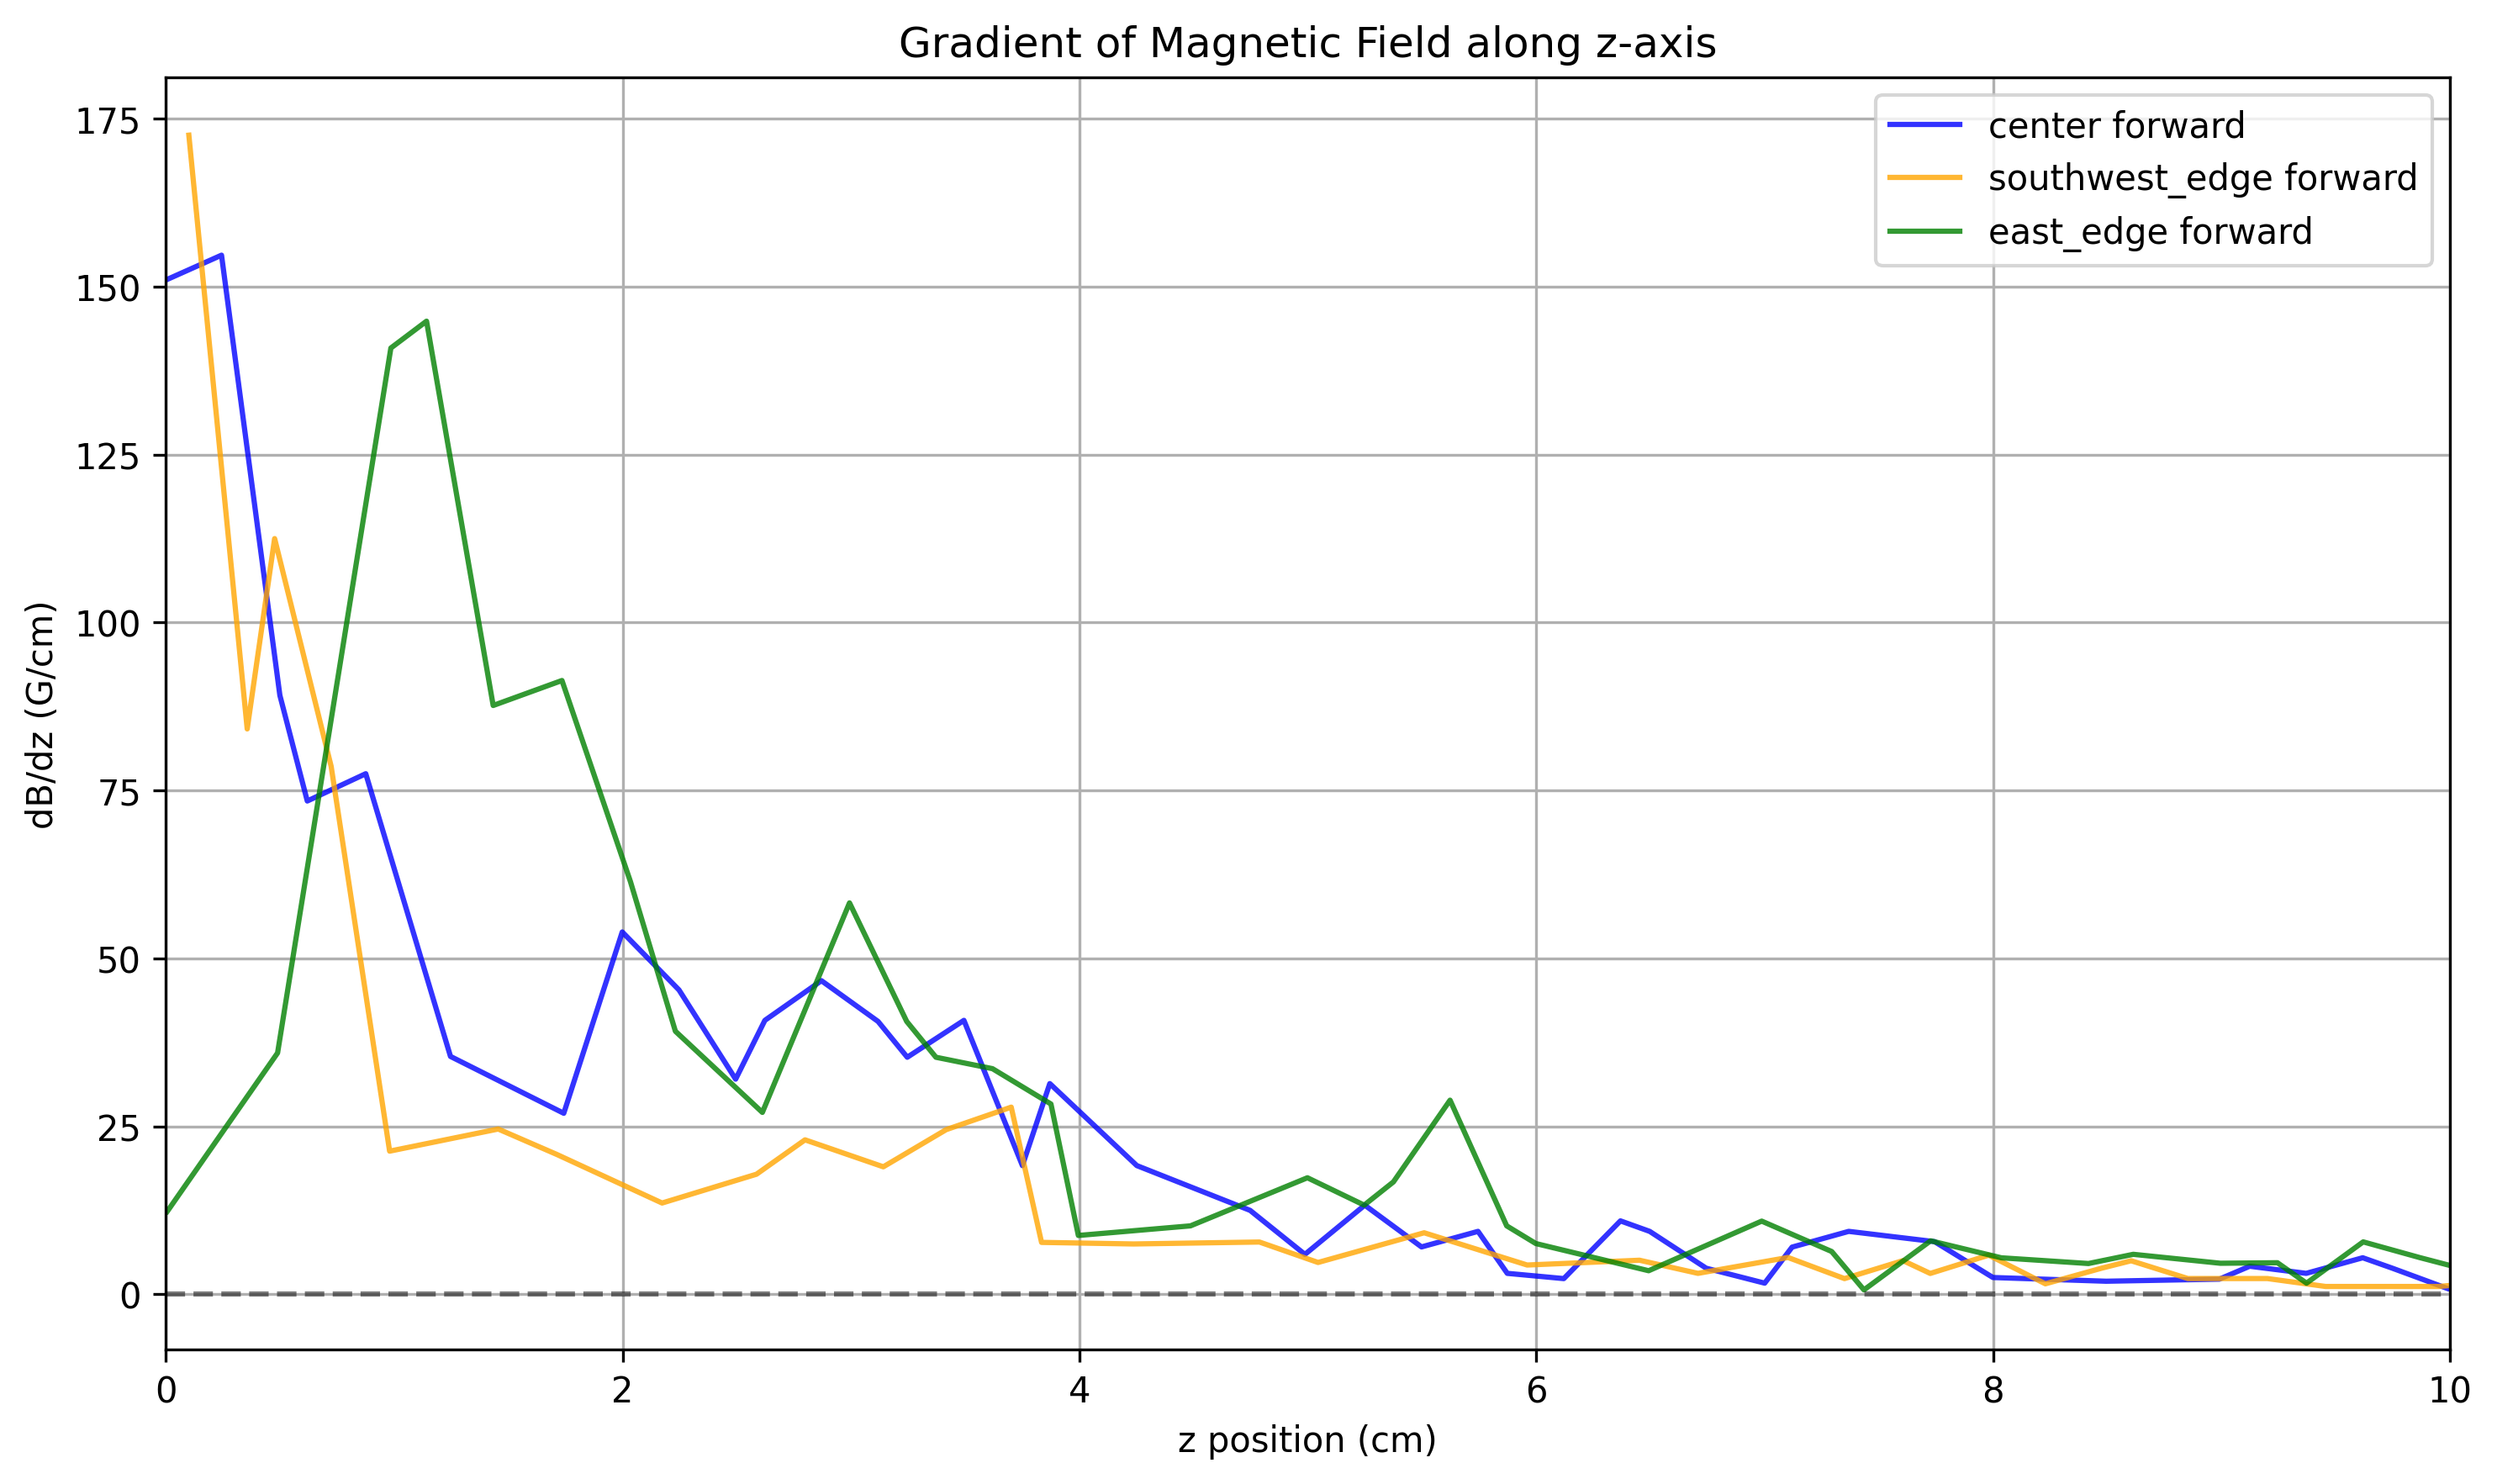
\includegraphics[width=0.90\textwidth]{Assets/gradB.png}
	}
	\hfill
	\subfigure[$B\nabla B$ product along the path.\label{fig:b_gradb}]{
		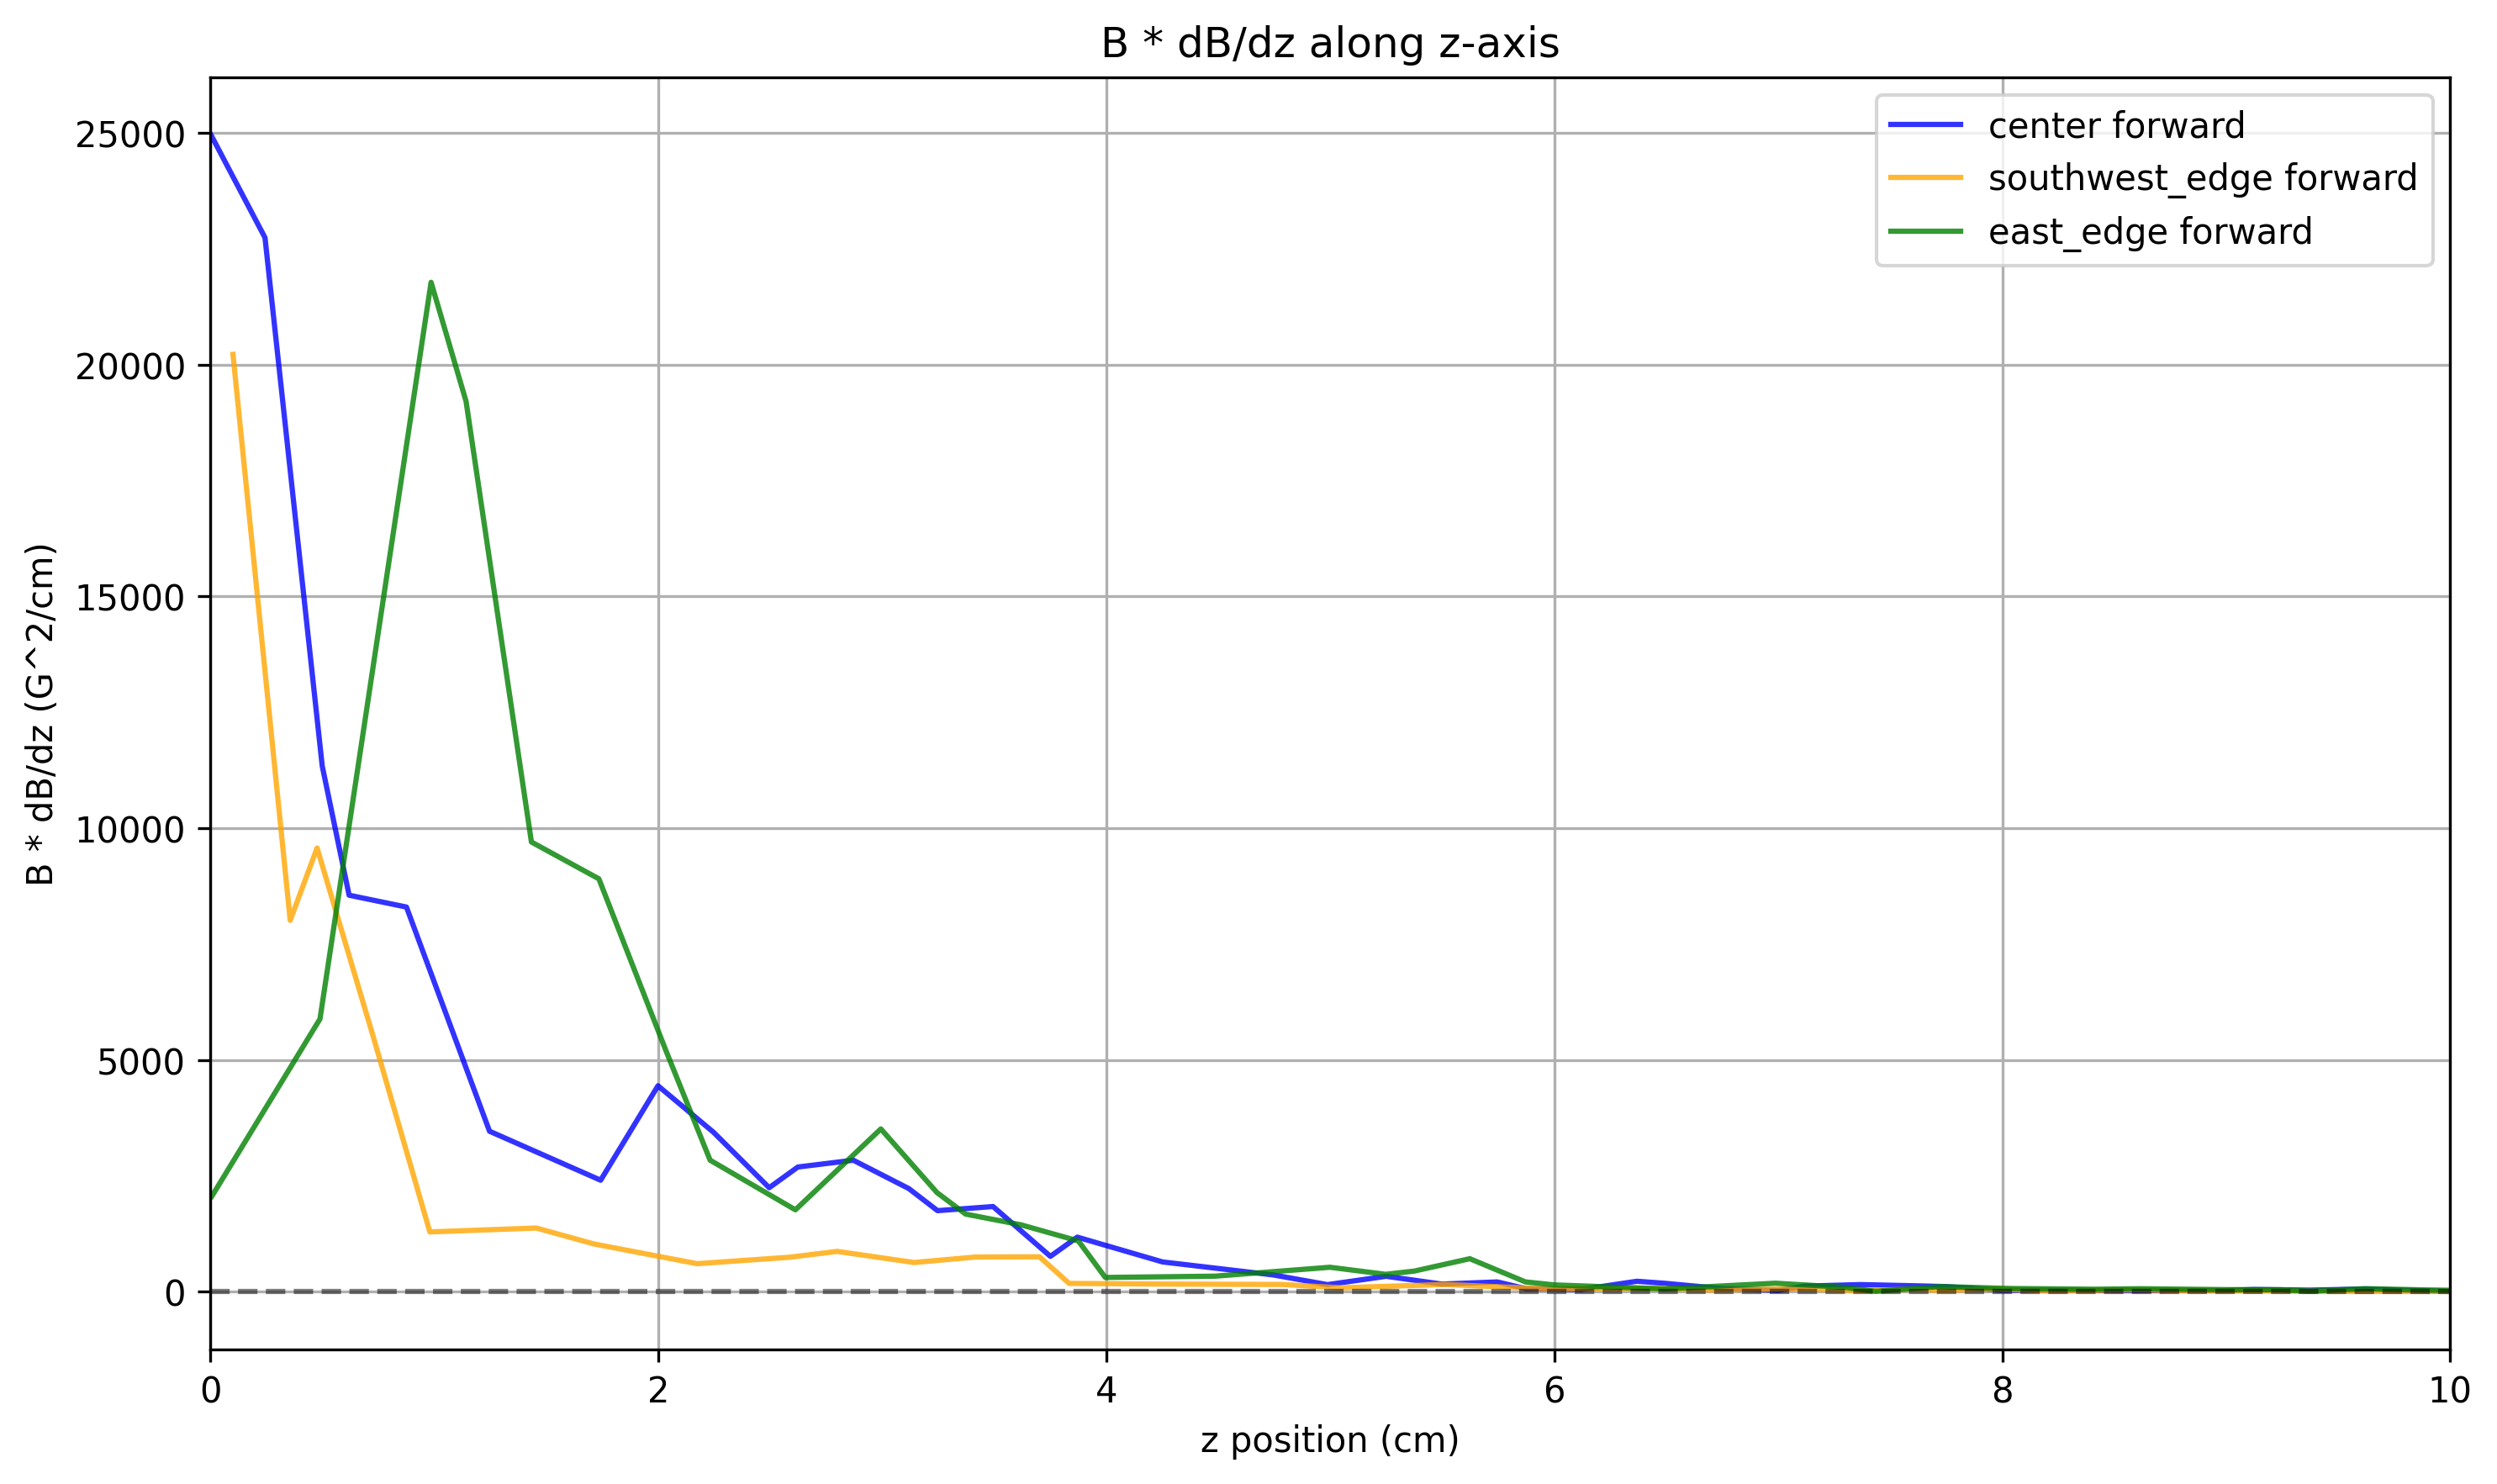
\includegraphics[width=0.90\textwidth]{Assets/BgradB.png}
	}
	
	\caption[Spatial magnetic gradients and $B\nabla B$ product]{Computed magnetic field gradients and the $B\nabla B$ product used for translational force characterization.}
	\label{fig:gradb_pair}
\end{figure}

In the translational experiment, the current applied to our solenoid was varied, and the magnetic field was measured in specific points within 7 to 8 cm away from the solenoid, this lead to a different results which are the points of equilibrium of the pendulum. These results are meaningful and will be used in section \ref{sec:res_labscale-Translational}. 

\begin{figure}[htb!]
	\centering
	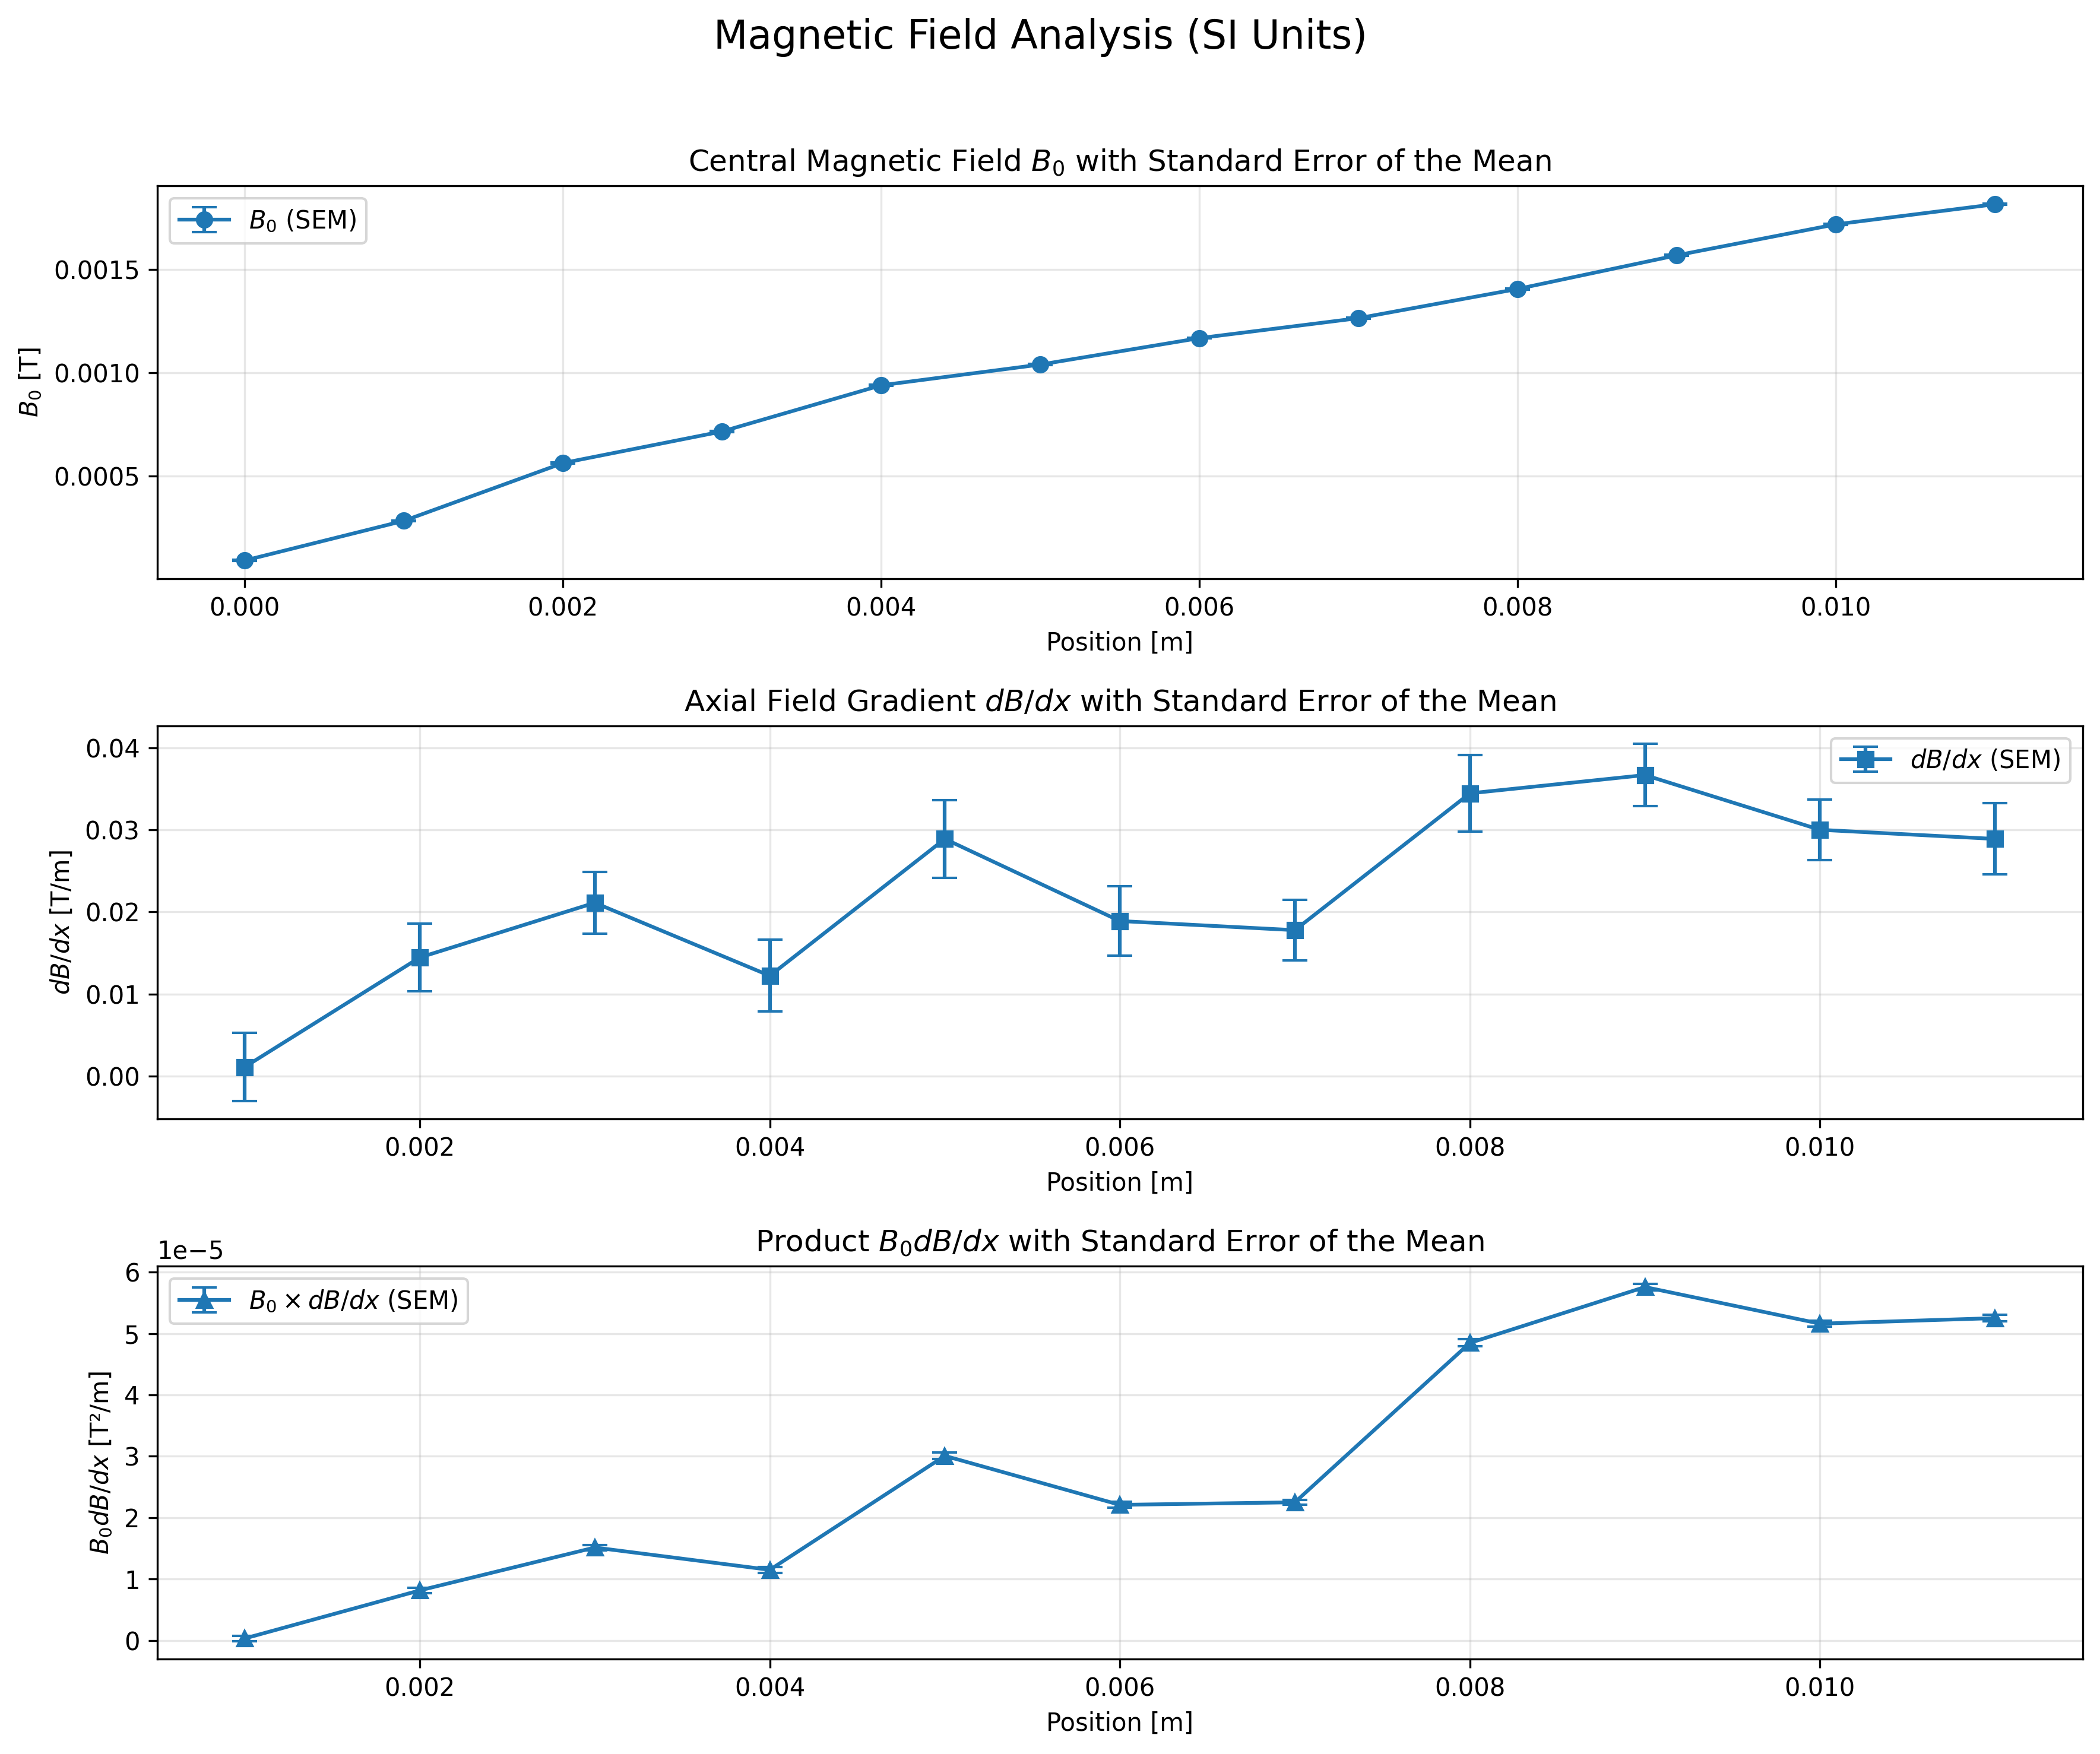
\includegraphics[width=0.9\textwidth]{Assets/magField_behavior_SI.png}
	\caption[Magnetic field behavior in SI units]{Central magnetic field $B_0$, axial field gradient $dB/dx$, and their product $B_0 dB/dx$ as functions of position along the magnet axis. All quantities are shown in SI units (Tesla, T/m, and T$^2$/m, respectively) with error bars representing the standard error of the mean (SEM).}
	\label{fig:EquilibriumPointsField}
\end{figure}

As the measurement of magnetic field was done by varying current and not distance the magnetic field plots looks different of that showed by Figures \ref{fig:bfield_time_z} and \ref{fig:gradb_pair}. Figure \ref{fig:EquilibriumPointsField} shows three plots, which corresponds to the three operations needed to make the field side of Equation \ref{eq:forFit}. As highlighted, in this instance the x-axis, position, refers to the position of the pendulum's end with respect of its gravitational equilibrium point, and each point was taken with a different current applied to the solenoid while the pole remained stationary.

\subsection{Mapping for 3T Siemens Magnetom\textsuperscript{\texttrademark} \gls{mri} scanner}


